\documentclass{beamer}
\usepackage[spanish]{babel}
\usepackage[latin1]{inputenc}
\usepackage{multicol} % indice en 2 columnas
\usepackage{centernot}
\usepackage{amsmath}% http://ctan.org/pkg/amsmath

\usepackage{color}


\usepackage{graphicx}
\graphicspath{ {im/} }


\newcommand{\notimplies}{%
  \mathrel{{\ooalign{\hidewidth$\not\phantom{=}$\hidewidth\cr$\implies$}}}}


\usetheme{Warsaw}
%\usecolortheme{crane}
\useoutertheme{shadow}
\useinnertheme{rectangles}

\setbeamertemplate{navigation symbols}{} % quitar simbolitos



\title[Tema 7 - Introducci\'on a la matem\'atica discreta]{Matem\'atica discreta}
\subtitle{Estudios de Ingenier\'ia}
\author[https://frogames.es]{
Juan Gabriel Gomila%$^{1}$  \and E. Eva$^{2}$ \and S. Serpiente$^{3}$
}
\institute[Frogames]{
 % $^{1-2}$
 Frogames
   \and
  \texttt{https://frogames.es}
}
\date{\today}


\AtBeginSection{
\begin{frame}
  \begin{multicols}{2}
  \tableofcontents[currentsection]   
\end{multicols}
\end{frame}
}

\AtBeginSubsection{
\begin{frame}
  \begin{multicols}{2}
  \tableofcontents[currentsection,currentsubsection]
\end{multicols}
\end{frame}
}



%empieza aqui


\begin{document} 

\frame{\titlepage}

\begin{frame}
  \frametitle{\'Indice}
  \tableofcontents
\end{frame}

\section{Teor\'ia b\'asica de conjuntos}
\subsection{El concepto de conjunto}
\begin{frame}
\frametitle{El concepto de conjunto}
\begin{block}{Definici\'on}
Un conjunto es una colecci\'on de objetos. Los objetos que forman parte de un conjunto determinado se denominan elementos del conjunto.
\end{block}


Ejemplos de conjuntos son la colecci\'on de todos los estudiantes del grado de telem\'atica, la colecci\'on de todos los n\'umeros enteros pares, etc\'etera.
\end{frame}



\begin{frame}
\frametitle{Conjuntos por extensi\'on}
Para describir un conjunto con un n\'umero finito de elementos se puede hacer por \textbf{extensi\'on}; es decir, mediante un listado de sus elementos entre claves como por ejemplo$\{1,2,3,4,5\}$.

No es importante el orden en que se escriben los elementos. As\'i $\{1, 2, 3, 4\}$ y $\{4, 3, 2, 1\}$ representan el mismo conjunto.


No se ha de tener en cuenta si la lista tiene alg\'un elemento repetido. El conjunto $\{1, 2, 3, 4, 2\}$ es el mismo que el anterior.
\end{frame}


\begin{frame}
\frametitle{Como denotar un conjunto}
Se emplear\'an letras may\'usculas para designar los conjuntos y letras min\'usculas para designar sus elementos.

Para indicar que $x$ es un elemento de $A$, se escribir\'a $x\in A$ ($x$ perteneciente a $A$).

Para indicar que $x$ no es un elemento de $A$, se escribir\'a $x\notin A$ ($x$ no pertenece a $A$).
\end{frame}


\begin{frame}
\frametitle{Conjuntos por compresi\'on}
Tambi\'en se pueden describir los conjuntos por \textbf{compresi\'on}; es decir, espec\'ificamente una propiedad qu determina exactamente sus elementos. Se escribir\'a como:
\[A=\{x\ |\ p(x)\}\]
Por ejemplo:
\[A=\{x\ | \ x \textrm{\ es\ entero\ positivo\ menor\ que\ 5}\}\]
Representa al conjunto $A=\{1,2,3,4\}$,
\end{frame}



\begin{frame}
\frametitle{Un conjunto sin elemento}
\begin{block}{El conjunto vac\'io}
El conjunto que no tiene ning\'un elemento se denota por $\emptyset$ y se denomina conjunto vac\'io. Por ejemplo:
\[\{x\in\mathbb R\ | \ x^2 = -2\} = \emptyset\]
\end{block}
\end{frame}




\begin{frame}
\frametitle{Igualdad de conjuntos}
\begin{block}{Definici\'on}
Dos conjuntos $A$ y $B$ son iguales cuando tienen exactamente los mismo elementos; es decir, cuando todo elemento de $A$ es elemento de $B$ y todo elemento de $B$ es elemento de $A$. 

Cuando $A$ y $B$ son iguales se denota como $A=B$.
\end{block}
\end{frame}


\begin{frame}
\frametitle{Subconjuntos}
\begin{block}{Definici\'on}
D\'icese que un conjunto $A$ es un subconjunto de $B$ si todo elemento de $A$ es elemento de $B$ y se escribir\'a como $A\subseteq B$, notaci\'on que significa que $A$ est\'a contenido en $B$, o que $B$ contiene a $A$.
\end{block}
\end{frame}


\begin{frame}
\frametitle{El conjunto universal}
\begin{block}{Definici\'on}
Siempre que se hable de conjuntos, se supondr\'a que son subconjuntos de un conjunto universal $U$ que los contiene a todos.
\end{block}
El conjunto universal contiene todos los conjuntos a los cuales se hace referencia en un ejercicio o resultado.
\end{frame}




\begin{frame}
\frametitle{Ejemplos de subconjuntos}
\begin{itemize}
\item $\mathbb N \subseteq \mathbb Z \subseteq \mathbb Q\subseteq \mathbb R\subseteq \mathbb C$.
\item $\mathbb Z^{+} = \{x\in\mathbb Z: x>0\} \subseteq \mathbb Z$
\item Si $A$ es un conjunto cualquiera, entonces $\emptyset\subseteq A$ y $A\subseteq A$. Estos dos se denominan subconjuntos triviales de $A$.
\item Si $A$ es un conjunto cualquiera y $B=\{A,\{A\}\}$, entonces $A\in B$, $\{A\}\in B$, $\{A\}\subseteq B$ pero en cambio $A\not\subseteq B$.
\end{itemize}
Se puede comprobar f\'acilmente que $A=B\Longleftrightarrow A\subseteq B$ y $B\subseteq A$ (Ejercicio).
\end{frame}

\subsection{Operaciones con conjuntos}


\begin{frame}
\frametitle{Operaciones con conjuntos}
Se ver\'an algunas operaciones b\'asicas de conjuntos. Las operaciones entre conjuntos y las propiedades que verifican estas operaciones se pueden ilustrar mediante \textbf{diagramas de Venn}. Un diagrama de Venn es una representaci\'on gr\'afica de conjuntos en el plano. El conjunto universal $U$ se representa por el interior de un rect\'angulo y los otros subconjuntos son representados por c\'irculos en el rect\'angulo.
\end{frame}


\begin{frame}
\frametitle{Operaciones con conjuntos}
\begin{block}{Uni\'on de conjuntos}
Sean $A$ y $B$ conjuntos, se define su uni\'on como el conjunto de todos los elementos que pertenecen a $A$ o a $B$.
\[A\cup B = \{x:x\in\ A\ o \ x\in\ B\}\]
\end{block}
Si $A=\{a,b,c,d\}$ y $B = \{a,b,g,e,h\}$, entonces:
\[A\cup B = \{ a,b,c,d,g,e,h\}\]
\end{frame}

\begin{frame}
\frametitle{Operaciones con conjuntos}
\begin{block}{Intersecci\'on de conjuntos}
Sean $A$ y $B$ conjuntos, se define su intersecci\'on como el conjunto de todos los elementos que pertenecen al mismo tiempo a $A$ y a $B$.
\[A\cap B = \{x:x\in\ A\ y \ x\in\ B\}\]
\end{block}
Si $A=\{a,b,c,d\}$ y $B = \{a,b,g,e,h\}$, entonces:
\[A\cap B = \{ a, b\}\]
\end{frame}


\begin{frame}
\frametitle{Operaciones con conjuntos}
La uni\'on y la intersecci\'on de conjuntos tambi\'en se puede definir para tres o m\'as conjuntos de la manera siguiente:

\[A\cup B \cup C = \{x:x\in\ A\ o \ x\in\ B\ o \ x\in\ C\}\]
\[A\cap B \cap C = \{x:x\in\ A\ y \ x\in\ B\ y \ x\in\ C\}\]
Y por tanto, la uni\'on y la intersecci\'on de un n\'umero finito de conjuntos se define como:
\[\displaystyle\bigcup_{i=1}^n A_i = A_1\cup A_2\cup \cdots \cup A_n = \{x:x\in\ A_i\ para\ algun\ i\}\]
\[\displaystyle\bigcap_{i=1}^n A_i = A_1\cap A_2\cap \cdots \cap A_n = \{x:x\in\ A_i\ para\ todo \ i\}\]
\end{frame}



\begin{frame}
\frametitle{Operaciones con conjuntos}
\begin{block}{Conjuntos disjuntos}
D\'icese que dos conjuntos $A$ y $B$ son disjuntos cuando no tienen elementos en com\'un; es decir, cuando:
\[A\cap B = \emptyset\]
\end{block}
\end{frame}




\begin{frame}
\frametitle{Operaciones con conjuntos}
\begin{block}{Diferencia de conjuntos}
Sean $A$ y $B$ conjuntos, se define la diferencia $A-B$ como el conjunto de elementos de $A$ que no pertenecen a $B$.
\[A- B = \{x:x\in A \ y \ x\notin B\}\]
\end{block}
Si $A=\{a,b,c,d\}$ y $B = \{a,b,g,e,h\}$, entonces:
\[A-B = \{c,d\}\]
\[B-A = \{g,e,h\}\]
\end{frame}


\begin{frame}
\frametitle{Operaciones con conjuntos}
\begin{block}{Complementario de un conjunto}
Sea $U$ un conjunto universal que contiene un conjunto $A$, entonces el conjunto $U-A$ se denomina complemento o complementario de $A$ y se denota como $A^c$. As\'i:
\[A^c = \{x:x\notin A\}\]
\end{block}
Si $U=\mathbb{Z}$  y $A=\{x:x\ pares\}$, entonces:
\[A^c = \{x:x\ impares\}\]
\end{frame}


\begin{frame}
\frametitle{Operaciones con conjuntos}
\begin{block}{Diferencia sim\'etrica}
Sean $A$ y $B$ conjuntos, se define la diferencia sim\'etrica de $A$ y $B$ como el conjunto uni\'on de los elementos de $A$ que no pertenecen a $B$ y los elementos de $B$ que no pertenecen a $A$.
\[A \oplus B = \{x:(x\in A \ y \ x \notin B)\ o\ (x\in B\ y \ x\notin A )\}\]
\end{block}
Es f\'acil notar que: 
\[A \oplus B = (A-B)\cup (B-A)\]
Si $A=\{a,b,c,d\}$ y $B = \{a,b,g,e,h\}$, entonces:
\[A \oplus B = \{c,d,g,e,h\}\]
\end{frame}




\begin{frame}
\frametitle{Operaciones con conjuntos}
\begin{block}{Partes de un conjunto}
Sea $A$ un conjunto. El conjunto de todos los subconjuntos de $A$ se denomina conjunto de partes de $A$ (o conjunto potencia de $A$) y se denota como $\mathcal{P}(A)$.
\[\mathcal{P}(A) = \{X:X\subseteq A\}\]
\end{block}
Si $A=\{a,b,c\}$, entonces:
\[\mathcal{P}(A) = \{\emptyset, \{a\},\{b\},\{c\}, \{a,b\}, \{a,c\},\{b,c\},\{a,b,c\} \}\]
\end{frame}

\subsection{Propiedades}

\begin{frame}
\frametitle{Propiedades}
En las diapositivas siguientes se muestran algunas de las propiedades algebraicas que satisfacen las operaciones de conjuntos, donde $A,B,C$ son subconjuntos de un conjunto universal $U$.
\end{frame}



\begin{frame}
\frametitle{Propiedades}
\begin{block}{Conmutativas}
\[A\cup B = B\cup A\]
\[A\cap B = B\cap A\]
\end{block}

\begin{block}{Asociativas}
\[(A\cup B)\cup C = A\cup (B\cup C)\]
\[(A\cap B)\cap C = A\cap (B\cap C)\]
\end{block}

\end{frame}





\begin{frame}
\frametitle{Propiedades}
\begin{block}{Idempotencia}
\[A\cup A = A\]
\[A\cap A = A\]
\end{block}

\begin{block}{Involutiva}
\[(A^c)^c = A\]
\end{block}

\end{frame}




\begin{frame}
\frametitle{Propiedades}
\begin{block}{Distributivas}
\[A\cup (B \cap C) = (A\cup B)\cap (A\cup C)\]
\[A\cap (B \cup C) = (A\cap B)\cup (A\cap C)\]
\end{block}

\begin{block}{Leyes de De Morgan}
\[(A\cup B)^c = A^c\cap B^c\]
\[(A\cap B)^c = A^c\cup B^c\]
\end{block}

\end{frame}



\begin{frame}
\frametitle{Propiedades}
\begin{block}{Absorci\'on}
\[A\cup (A \cap B) = A\]
\[A\cap (A \cup B) = A\]
\end{block}

\begin{block}{Elementos absorbentes}
\[A\cup U = U\]
\[A\cap \emptyset = \emptyset\]
\end{block}

\end{frame}




\begin{frame}
\frametitle{Propiedades}
\begin{block}{Elemento neutro}
\[A\cup \emptyset = A\]
\[A\cap U = A\]
\end{block}

\begin{block}{Complementos}
\[A\cup A^c = U\]
\[A\cap A^c = \emptyset\]
\[ \emptyset^c = U\]
\[ U^c = \emptyset\]
\end{block}

\end{frame}



\subsection{Conjunto finito. Principio de la adici\'on}

\begin{frame}
\frametitle{Conjuntos finitos}
\begin{block}{Conjunto finito}
Un conjunto $A$ es finito si contiene exactamente $m$ elementos distintos donde $m$ es un entero no negativo. Si un conjunto no es finito, es infinito.


Si $A$ es finito se denota como $|A|$ o como $card(A)$ al n\'umero de elementos de $A$.
\end{block}

El conjunto $\emptyset$ es finito y $|\emptyset | = 0$. El conjunto de letras del alfabeto castellano es finito, y el conjunto de todos los enteros positivos e impares es infinito.

Si $A$ es un conjunto con $|A|=m$, entonces $|\mathcal{P}(A)| = 2^m$.

\end{frame}



\begin{frame}
\frametitle{Principio de la adici\'on}
\begin{block}{Teorema}
Si $A$ y $B$ son conjuntos finitos, entonces $A\cup B$ y $A\cap B$ son finitos y:
\[|A\cup B | = |A| + |B| - |A\cap B|\]
\end{block}
En particular si $A\cap B = \emptyset$, entonces $|A\cup B| = |A|+|B|$.
\end{frame}




\begin{frame}
\frametitle{Principio de adici\'on}

En el caso de la uni\'on de tres conjuntos, la f\'ormula que devolver\'a su cardinal es:
\[|A\cup B \cup C| = |A| + |B| + |C| - |A\cap B| - |A\cap C| - |B\cap C| + |A\cap B \cap C|\]
En el caso de la uni\'on de $n$ conjuntos, la f\'ormula que devolver\'a su cardinal es:
\[|A_1\cup \cdots \cup A_n| = \alpha_1-\alpha_2+\alpha_3-\cdots + (-1)^(n-1)\alpha_n\]
Donde cada $\alpha_i$ es la suma de todos los cardinales de todas las intersecciones de $i$ conjuntos de los $n$ conjuntos dados. 
\end{frame}

\section{\'Algebra de Boole}

\begin{frame}
\frametitle{\'Algebra de Boole}
El \'algebra de Boole es una estructura matem\'atica que, como tal, aparece en muchas situaciones. En particular, el \'algebra de Boole tiene aplicaci\'on en la s\'intesis de redes de conmutaci\'on, en el estudio de circuitos digitales y en el an\'alisis y programaci\'on mediante ordenador.
\end{frame}

\subsection{Definici\'on de \'algebra de Boole}

\begin{frame}
\frametitle{\'Algebra de Boole}
\begin{block}{Definici\'on}
Sea $\mathcal{B} = <B,+,*,{}^-,0,1>$ donde:

\begin{itemize}
\item $B$ es un conjunto no vac\'io ($B\neq \emptyset)$,
\item $0,1\in B$ con $0\neq 1$
\item $+$ y $*$ son operaciones binarias:
\begin{multicols}{2} 

  \[
  \begin{array}{@{}r@{\;}c@{\;}c@{\;}l@{}}
    +: & B\times B & \rightarrow & B,   \\
       & (a,b) & \mapsto     & a+b.
  \end{array}
\]

  \[
  \begin{array}{@{}r@{\;}c@{\;}c@{\;}l@{}}
    *: & B\times B & \rightarrow & B,   \\
       & (a,b) & \mapsto     & a*b.
  \end{array}
\]
\end{multicols}
\item ${}^-$ es una operaci\'on unaria:

  \[
  \begin{array}{@{}r@{\;}c@{\;}c@{\;}l@{}}
    {}^-: & B & \rightarrow & B,   \\
       & a & \mapsto     & \bar{a}.
  \end{array}
\]
\end{itemize}
\end{block}
\end{frame}



\begin{frame}
\frametitle{\'Algebra de Boole}
D\'icese que $\mathcal{B}$ tiene estructura de \'algebra de Boole si:

\begin{block}{A1}
Las operaciones $+$ y $*$ son asociativas $\forall\ a,b,c\in B$
\[(a+b)+c = a+(b+c)\]
\[(a*b)*c = a*(b*c)\]
\end{block}


\begin{block}{A2}
Las operaciones $+$ y $*$ son conmutativas $\forall\ a,b\in B$
\[a+b = b+a\]
\[a*b = b*a\]
\end{block}
\end{frame}


\begin{frame}
\frametitle{\'Algebra de Boole}
\begin{block}{A3}
Cada operaci\'on binaria tiene elemento neutro $\forall a\in B$
\[\exists\ 0\in B :\ a+0 = 0+a = a\]
\[\exists\ 1\in B :\ a*1 = 1*a = a\]
\end{block}


\begin{block}{A4}
Para cada elemento $a\in B$ existe un \'unico elemento $\bar{a}\in B$ denominado complementario de $a$ tal que 
\[a+\bar{a} = 1;\ \ a*\bar{a} = 0\]
\end{block}
\end{frame}

\begin{frame}
\frametitle{\'Algebra de Boole}
\begin{block}{A5}
Cada operaci\'on binaria es distributiva respecto de la otra $\forall\ a,b,c\in B$
\[a*(b+c) = a*b+a*c\]
\[a+(b*c) = (a+b)*(a+c)\]
\end{block}

Estas cinco parejas de propiedades se conocen como los axiomas del \'algebra de Boole. Cualquier otra propiedad de un \'algebra de Boole se puede deducir a partir de las anteriores.
\end{frame}




\begin{frame}
\frametitle{\'Algebra de Boole}
Les operaciones $+,*$ y ${}^-$  se denominan suma, producto y complementario respectivamente. En ausencia de par\'entesis ${}^-$ tiene preferencia sobre $*$ y $*$ sobre $+$. Usualmente se omitir\'a el s\'imbolo $*$, as\'i para escribir $a*b$ lo haremos como $ab$.


El elemento neutro de la suma se denomina elemento $cero$ y el elemento neutro del producto se denomina elemento $unidad$.

\end{frame}




\begin{frame}
\frametitle{Ejemplos de \'algebras de Boole}
\begin{block}{Ejemplo 1}
Consid\'erese un conjunto $U$ finito y $U\neq \emptyset$. El conjunto $\mathcal{P}(U)$ con las operaciones: 
\begin{itemize}
\item $\cup$ uni\'on de conjuntos, 
\item $\cap$ intersecci\'on de conjuntos,
\item ${}^c$ complementario de un conjunto 
\end{itemize}
Tiene estructura de \'algebra de Boole.

El neutro de la uni\'on es el conjunto vac\'io $\emptyset$ y el neutro de la intersecci\'on es el conjunto $U$.

\end{block}
\end{frame}





\begin{frame}
\frametitle{Ejemplo de \'algebras de Boole}
\begin{block}{Ejemplo 2}
Sea $D_{70} = \{1,2,5,7,10,14,35,70\}$ el conjunto formado por los divisores de $70$. Si se define en $D_{70}$ las siguientes operaciones: 
\begin{itemize}
\item $a+b = mcm(a,b)$, 
\item $a*b = mcd(a,b)$,
\item $\bar{a} = 70/a$ 
\end{itemize}
Entonces $D_{70}$ tiene estructura de \'algebra de Boole con $1$ como elemento cero y $70$ como elemento unidad.
\end{block}
\end{frame}




\begin{frame}
\frametitle{Ejemplos de \'algebras de Boole}
\begin{block}{Ejemplo 3}
Sea $B= \{0,1\}$ con las operaciones binarias $+$ y $*$ definidas por:  

\begin{multicols}{2}
\begin{tabular}{ |p{1cm}|p{0.8cm}|p{0.8cm}|  }
 \hline
+&1&0 \\
 \hline
 1&1&1 \\
0 & 1 &  0 \\
 \hline
\end{tabular}


\begin{tabular}{ |p{1cm}|p{0.8cm}|p{0.8cm}|  }
 \hline
$*$&1&0 \\
 \hline
 1&1&0 \\
0 & 0 &  0 \\
 \hline
\end{tabular}
\end{multicols}
Y la operaci\'on unaria ${}^-$ definida por $\bar{0} = 1$, $\bar{1} = 0$. Entonces $\mathcal{B} = <0,1,+,*,{}^->$ es un \'algebra de Boole, denominada \textbf{\'algebra de Boole binaria}.

\end{block}
\end{frame}


\begin{frame}
\frametitle{Principio de dualidad}
\begin{block}{Principio}
En una \'algebra de Boole toda propiedad que se pueda deducir de lo axiomas o de cualquier otra propiedad derivada de ellos, da otra propiedad que se obtiene intercambiando:
\begin{itemize}
\item les operaciones suma y producto, 
\item los s\'imbolos 0 y 1
\end{itemize}
La propiedad que se obtiene de esta manera recibe el nombre de \textbf{propiedad dual} de la inicial.
\end{block}

\end{frame}

\begin{frame}
\frametitle{Principio de dualidad}

Por ejemplo, la propiedad dual de: 
\[(1+a)(b+0) = b\]
Es:
\[(0a)+(b1) = b\]
El principio de dualidad es consecuencia de la propia estructura del \'algebra de Boole, ya que cada par de propiedades, en su definici\'on, vienen dadas por una propiedad y su dual.
\end{frame}

\subsection{Propiedades en un \'algebra de Boole}

\begin{frame}
\frametitle{Propiedades}
Se puede demostrar matem\'aticamente que todo \'algebra de Boole finito es estructuralmente el mismo que un \'algebra de Boole de conjuntos. En este sentido todo \'algebra de Boole satisfar\'a las mismas propiedades que un \'algebra de Boole de conjuntos. As\'i, en la tabla siguiente se da la lista de propiedades que comparten un \'algebra de Boole finito, $\mathcal{B}$, y un \'algebra de Boole de conjuntos, $\mathcal{P}(U)$

\end{frame}




\begin{frame}
\frametitle{Propiedades}

\begin{figure}[h]
  \label{figura propiedades}
\centering
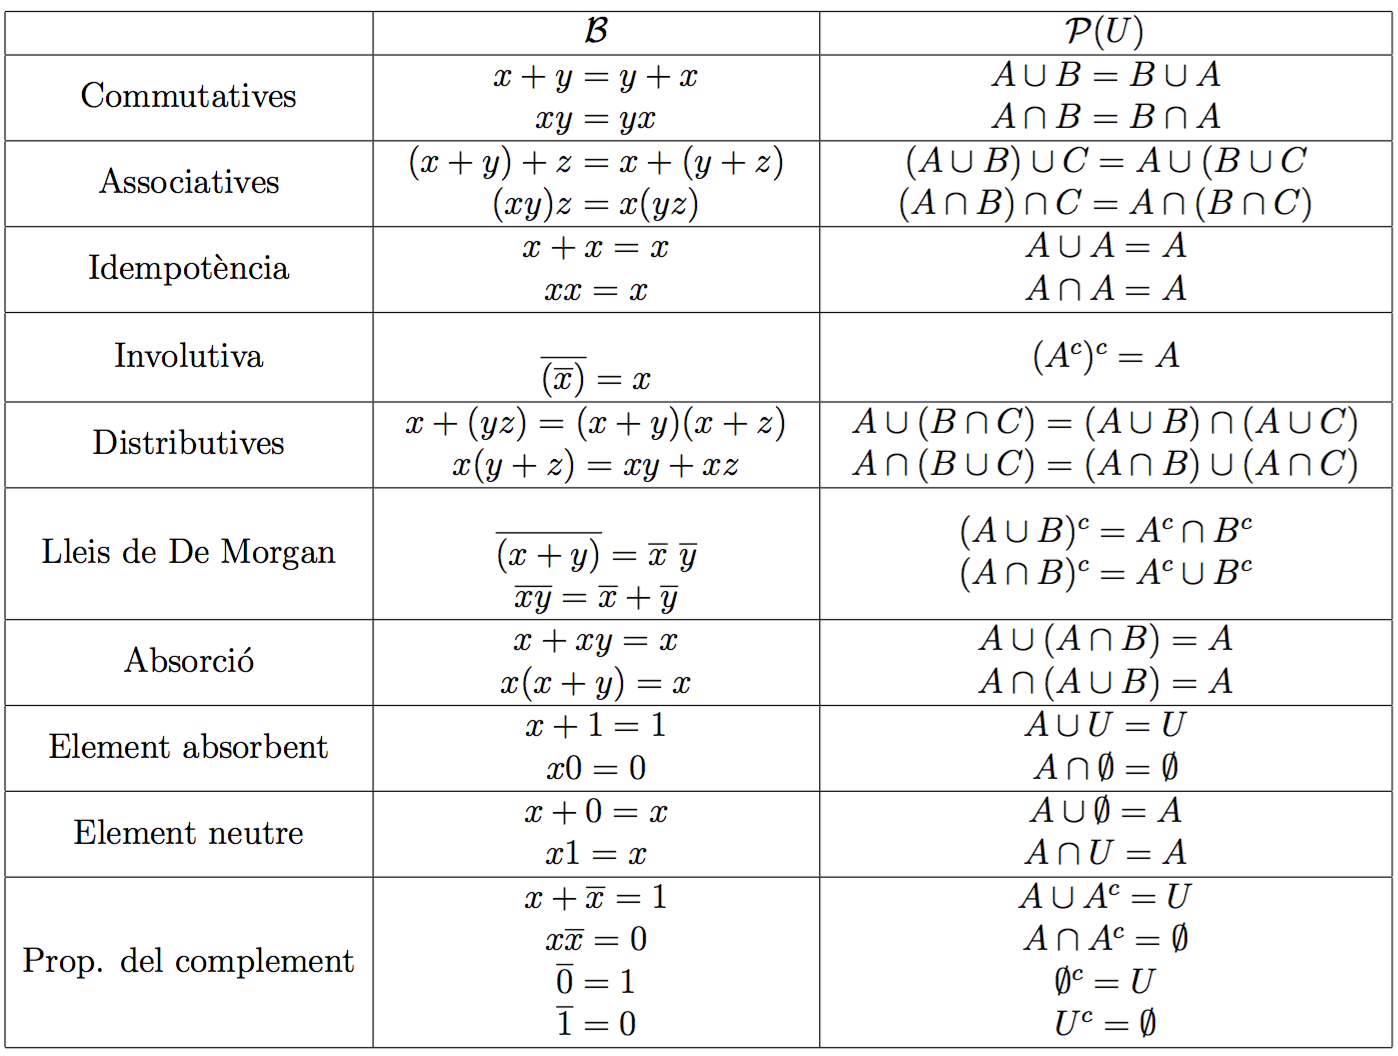
\includegraphics[height=7.0cm]{propietats}
\end{figure}

\end{frame}


\begin{frame}
\frametitle{Propiedades}
Se sabe que si un conjunto $A$ tiene $n$ elementos, entonces $|\mathcal{P}(A)| = 2^n$ y, debido a la relaci\'on que hay entre conjuntos y \'algebras de Boole, se puede enunciar el siguiente resultado:
\begin{block}{Teorema}
Todo \'algebra de Boole finito tiene $2^n$ elementos para alg\'un entero positivo $n$.
\end{block}
\end{frame}

\section{Funciones booleanas en el \'algebra de Boole binaria}
\subsection{Funciones booleanas}

\begin{frame}
\frametitle{Funciones booleanas}
Se considera a partir de ahora el \'algebra de Boole binaria donde $B=\{0,1\}$ y se denota como $B^n$ al producto cartesiano de $B$ con \'el mismo $n$ veces.
\[B^n = B\times B \times \cdots \times B = \{(x_1,x_2,\cdots,x_n):\ x_i \in \{0,1\}\forall \ i = 1,\cdots, n\}\]
Se denominan variaciones con repetici\'on de $n$ elementos diferentes tomados de $k$ en $k$ a las muestras ordenadas de $k$ elementos, los cuales se pueden repetir,  tomados de los $n$ elementos. 

Su n\'umero viene dado por $VR_{n,k} = n^k$.
\end{frame}

\begin{frame}
\frametitle{Funciones booleanas}
N\'otese que si $B=\{0,1\}$, entonces $|B^n| = 2^n$, as\'i
\[B^2 = \{(0,0), (0,1), (1,0), (1,1)\}\]
\[B^3 = \{(0,0,0), (0,0,1), (0,1,0), (1,0,0),\]\[(0,1,1),(1,0,1),(1,1,0),(1,1,1)\}\]
\end{frame}

\begin{frame}
\frametitle{Funciones booleanas}
\begin{block}{Definici\'on}
Se denomina funci\'on booleana definida en $B$ o funci\'on de conmutaci\'on l\'ogica a toda aplicaci\'on:
\[f:B^n\longrightarrow B\]
Tal que $f(x_1,x_2,\cdots,x_n)$ se puede expresar a partir de las operaciones definidas en $B$ realizadas sobre las variables $x_1,x_2,\cdots,x_n$.
\end{block}
Toda funci\'on booleana en $B=\{0,1\}$ se puede representar mediante tablas de valores o tablas de verdad. Las $n$ primeras columnas permiten representar los $2^n$ elementos de $B^n$ y la columna final indica el valor que asigna $f$ a cada $(x_1,x_2,\cdots,x_n)$. 
\end{frame}


\begin{frame}
\frametitle{Funciones booleanas}
\begin{block}{Ejemplo}
Calc\'ulense los valores de la funci\'on booleana
\[f(x_1,x_2,x_3) = x_1x_2+\bar{x_3}\]
\end{block}
Los valores de esta funci\'on vienen representados en la tabla siguiente:

\begin{figure}[h]
\label{fig:volum}
\centering
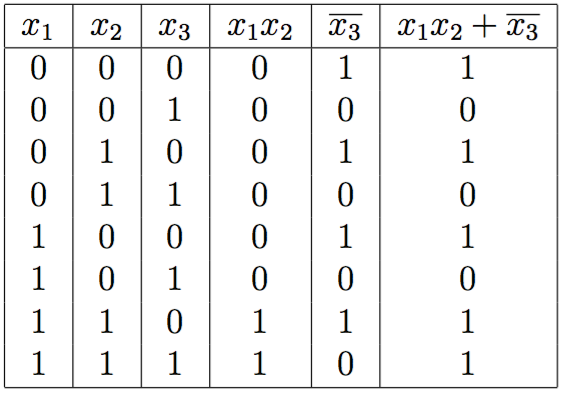
\includegraphics[height=3cm]{ex1}
\end{figure}
\end{frame}



\begin{frame}
\frametitle{N\'umero de funciones booleanes en el \'algebra de boole binaria}
El n\'umero de elementos del conjunto $B^n$ es $2^n$ y para cada uno de estos elementos una funci\'on booleana sobre $\{0,1\}$ puede tomar el valor $0$ o el valor $1$. Entonces:
\[\{f|\ f:B^n\longrightarrow B\} = VR_{2,2^n} = 2^{(2^n)}\]
As\'i para $n=2$, el n\'umero de funciones booleanas ser\'a $2^4 = 16$; para $n=3$, el n\'umero de funciones booleanas ser\'a $2^8 = 256$...
\end{frame}



\begin{frame}
\frametitle{N\'umero de funciones booleanas en el \'algebra de Boole binaria}
Las 16 funciones booleanas de dos variables son:
\begin{figure}[h]
\label{fig:volumen}
\centering
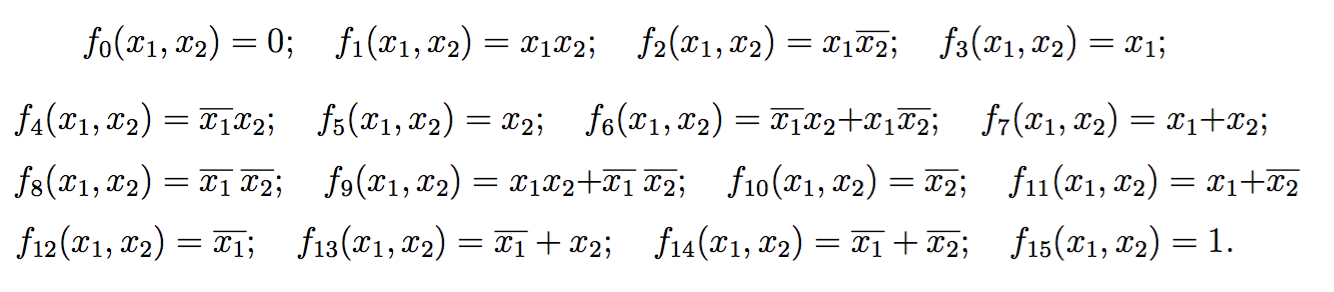
\includegraphics[width=\textwidth]{ex2}
\end{figure}
\begin{block}{Ejercicio}
Escr\'ibanse las tablas de valores de las funciones booleanas de dos variables.
\end{block}
\end{frame}

\begin{frame}
\frametitle{Funciones booleanas}
\begin{block}{Ejercicio}
Calc\'ulense los valores de la funci\'on booleana $F(x_1,x_2,x_3) = x_1x_2 + \bar x_3$
\begin{figure}[h]
\label{fig:volumen}
\centering
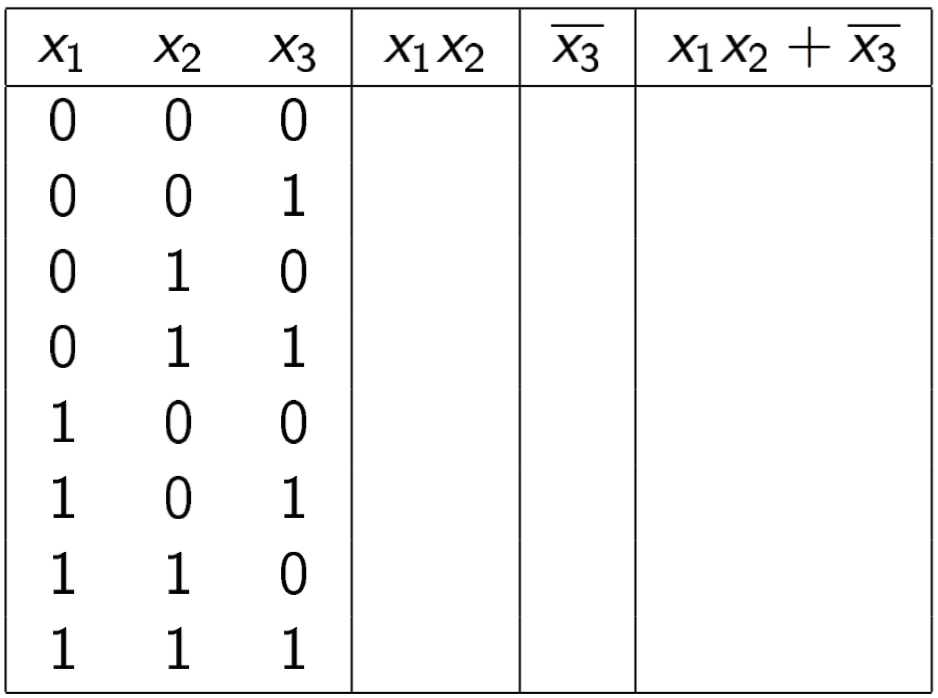
\includegraphics[height=4.5cm]{ex5_1}
\end{figure}

\end{block}
\end{frame}

\begin{frame}
\frametitle{Funciones booleanas}
\begin{block}{Ejercicio}
Soluci\'on:
\begin{figure}[h]
\label{fig:volumen}
\centering
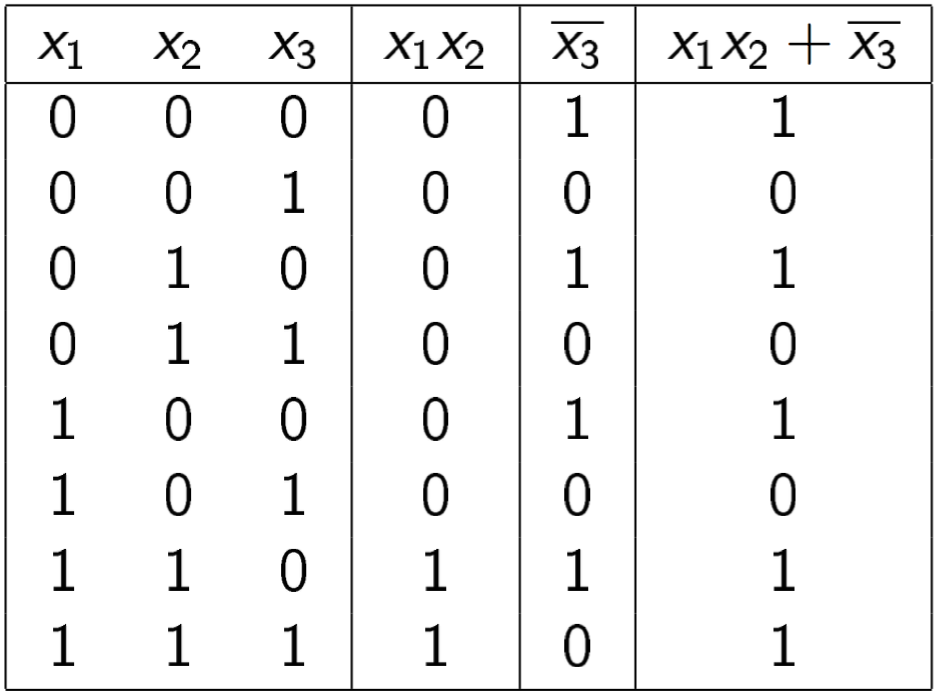
\includegraphics[height=4.5cm]{ex5_2}
\end{figure}

\end{block}
\end{frame}

\subsection{La forma can\'onica}

\begin{frame}
\frametitle{Formas can\'onicas}
\begin{block}{Minterm y Maxterm}
En $B^n$, el producto de $n$ variables diferentes complementadas o no, recine el nombre de \textbf{minterm}.
En $B^n$, la suma de $n$ variables diferentes complementadas o no, recibe el nombre de \textbf{maxterm}.
\end{block}
Por ejemplo, $B^4$, las expresiones $x_1x_2\bar{x_3}\bar{x_4}$, $\bar{x_1}x_2x_3\bar{x_4}$, son minterms.

Por ejemplo, en $B^3$, les expresiones $x_1+x_2+\bar{x_3}$, $\bar{x_1}+x_2+\bar{x_3}$, son maxterms.
\end{frame}


\begin{frame}
\frametitle{Formas can\'onicas}
\begin{block}{Proposici\'on}
Sea $f:B^n\longrightarrow B$ una funci\'on booleana, entonces:
\begin{itemize}
\item $f$ se puede expresar como una suma de minterms (suma de productos). Esta expresi\'on se denomina forma can\'onica disjuntiva de $f$.
\item $f$ se puede expresar como un producto de maxterms (producto de sumas). Esta expresi\'on se denomina forma can\'onica conjuntiva de $f$.
\end{itemize}
\end{block}
\end{frame}



\begin{frame}
\frametitle{Formas can\'onicas}
\begin{block}{Proposici\'on}
Sea $f:B^n\longrightarrow B$ una funci\'on booleana, entonces:
\begin{itemize}
\item Las formas can\'onicas de una funci\'on booleanas son \'unicas.
\item Dos funciones booleanas son equivalentes (son la misma funci\'on) si y solo si tienen las mismas formas can\'onicas.
\end{itemize}
\end{block}
\end{frame}



\subsection{Obtenci\'on de las formas can\'onicas}
\begin{frame}
\frametitle{Formas can\'onicas}
Las formas can\'onicas dee una funci\'on booleana se pueden obtener de dos maneras:
\begin{block}{1. A partir de una tabla de valores}
La \textbf{forma can\'onica disjuntiva} de $f:B^n\longrightarrow B$ se obtiene a partir de cada uno de los valores 1 que toma la funci\'on (un producto de todas las variables o sus complementos toman el valor 1 cuando \textbf{todos los factores toman el valor 1}).

As\'i el n\'umero de minterms en la forma disjuntiva es igual al n\'umero de unos (1) en la tabla de valores de $f$.
\end{block}
\end{frame}




\begin{frame}
\frametitle{Formas can\'onicas}

\begin{block}{1. A partir de una tabla de valores}
La \textbf{forma can\'onica conjuntiva} de $f:B^n\longrightarrow B$ se obtiene a partir de cada un de los valores 0 que toma la funci\'on (una suma de todas las variables o sus complementos toman el valor 0 cuando \textbf{todos los factores toman el valor 0}).

As\'i el n\'umero de maxterms en la forma conjuntiva es igual al n\'umero de ceros (0) en la tabla de valores de $f$.
\end{block}
\end{frame}


\begin{frame}
\frametitle{Formas can\'onicas}

\begin{block}{Ejercicios}
Obt\'enganse las formas can\'onicas disjuntiva y conjuntiva de la funci\'on $f:B^3\longrightarrow B$ dada por la tabla:

\begin{figure}[h]
\label{fig:volumen}
\centering
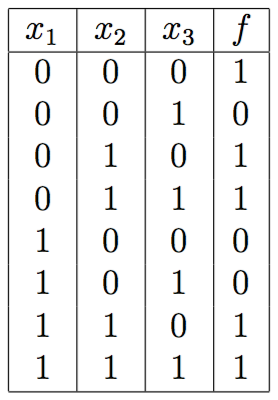
\includegraphics[height=4cm]{ex3}
\end{figure}
\end{block}
\end{frame}

\begin{frame}
\frametitle{Formas can\'onicas}

\begin{block}{Soluci\'on}
La forma can\'onica disjuntiva de $f$ ser\'a:
\[f(x_1,x_2,x_3) = \bar{x_1}\bar{x_2}\bar{x_3} + \bar{x_1}{x_2}\bar{x_3} + \bar{x_1}x_2x_3+x_1x_2\bar{x_3}+x_1x_2x_3\]
La forma can\'onica conjuntiva de $f$ ser\'a:
\[f(x_1,x_2,x_3) =(x_1+x_2+\bar{x_3})(\bar{x_1}+x_2+x_3)(\bar{x_1}+x_2+\bar{x_3})\]
\end{block}
\end{frame}


\begin{frame}
\frametitle{Formas can\'onicas}
\begin{block}{2. A partir de su expresi\'on en la f\'ormula}
Para obtener la \textbf{forma can\'onica disjuntiva} de $f:B^n\longrightarrow B$ interesa obtener una suma de productos, aunque estos t\'erminos no sean minterms.

La propiedad que lo suele permitir es la distributiva del producto respecto de la suma. Una vez obtenida la suma de productos, cada variable $x_j$ que no figura en un sumando se puede a\~nadir multiplic\'andola por 1, entonces $1=x_j+\bar{x_j}$ y, despu\'es se vuelve a aplicar la propiedad distributiva.

\end{block}
\end{frame}



\begin{frame}
\frametitle{Formas can\'onicas}
\begin{block}{2. A partir de su expresi\'on en la f\'ormula}
Para obtener la \textbf{forma can\'onica conjuntiva} de $f:B^n\longrightarrow B$ se va a transformar la expresi\'on inicial en producto de sumas. En este caso juega un papel esencial la propiedad distributiva de la suma respecto del producto.

Una vez se obtenga el producto de sumas, cada variable $x_j$ que no figura en un factor se puede a\~nadir sumando 0, haciendo $0=x_j\bar{x_j}$ y, despu\'es se vuelve a aplicar la propiedad distributiva.
\end{block}

En ambos casos, despu\'es de multiplicar por 1 o sumar 0 y aplicar las propiedades distributivas correspondientes se han de eliminar los minterms o maxterms repetidos aplicando la propiedad idempotente.
\end{frame}





\begin{frame}
\frametitle{Formas can\'onicas}
\begin{block}{Ejercicio}
Obt\'enganse las formas can\'onicas disjunta y conjuntiva de la funci\'on $f:B^3\longrightarrow B$ dada por: 
\[f(x,y,z) = \bar{x} + yz\]
\end{block}
\end{frame}




\begin{frame}
\frametitle{Formas can\'onicas}
\begin{block}{Soluci\'on en la forma disjuntiva}
\[f(x,y,z) = \bar{x} + yz =\]
Se introducen las variables que falten en cada sumando:
\[ \bar{x}(y+\bar{y})(z+\bar z) + (x+\bar x)yz = \]
Se aplica la propiedad distributiva:
\[\bar x yz + \bar xy\bar z + \bar x \bar y z + \bar x \bar y \bar z + xyz + \bar x y z\]
Se eliminan minterms repetidos gracias a la idempotencia:
\[\bar x yz + \bar xy\bar z + \bar x \bar y z + \bar x \bar y \bar z + xyz .\]

\end{block}
\end{frame}


\begin{frame}
\frametitle{Formas can\'onicas}
\begin{block}{Soluci\'on en la forma conjuntiva}
\[f(x,y,z) = \bar{x} + yz =\]
Se aplica la distributiva de la suma respecto del producto:
\[ (\bar x + y)(\bar x+z) = \]
Se a\~nade a cada factor las variables que falten:
\[ (\bar x + y +z\bar z)(\bar x+y\bar y+z) = \]
Se aplica la conmutativa de la suma seg\'un el factor:
\[ (\bar x + y +z\bar z)(\bar x+z+y\bar y) = \]
...
\end{block}
\end{frame}


\begin{frame}
\frametitle{Formas can\'onicas}
\begin{block}{Soluci\'on en la forma conjuntiva}
Se aplica la distributiva de la suma respecto del producto:
\[ (\bar x + y +z)(\bar x + y +\bar z)(\bar x+z+y)(\bar x+z+\bar y) = \]
Se aplica la conmutativa de la suma:
\[ (\bar x + y +z)(\bar x + y +\bar z)(\bar x+y+z)(\bar x+\bar y+z) = \]
Se eliminan los maxterms repetidos gracias a la idempotencia:
\[ (\bar x + y +z)(\bar x + y +\bar z)(\bar x+\bar y+z). \]
\end{block}
Es importante a\~nadir las variables en el orden en que figuren en la funci\'on: $x,y,z$.
\end{frame}




\subsection{Simplificaci\'on de variables booleanas}


\begin{frame}
\frametitle{Simplificaci\'on de variables booleanas}
El objetivo de esta secci\'on es la obtenci\'on de expresiones simplificadas de las funciones booleanas, tanto si su expresi\'on inicial es una de las formas can\'onicas como si no.

Los m\'etodos habituales de simplificaci\'on son tres: m\'etodo algebraico, m\'etodo gr\'afico (los mapas de Karnaugh) y el m\'etodo iterativo (m\'etodo de Quine-McCluskey).

Nosotros solo utilizaremos el m\'etodo algebraico y el m\'etodo gr\'afico.
\end{frame}




\begin{frame}
\frametitle{Simplificaci\'on de variables booleanas}
\begin{block}{M\'etodo algebraico}
Consiste en la utilizaci\'on de las propiedades generales v\'alidas en cualquier \'algebra de Boole. Las propiedades que facilitan el proceso de simplificaci\'on son:
\begin{itemize}
\item Complementario: $x+\bar x = 1;\ \  x\bar x = 0$
\item Idempotencia: $x+ x = x;\ \  x x = x$
\item Absorci\'on: $x+ xy = x;\ \  x( x+y) = x$
\item Ley de De Morgan: $\overline{x+y}  = \bar x\bar y ;\ \  \overline{xy} = \bar x + \bar y$
\item Distributivas: $xy+z = x(y+z);\ \ x+yz = (x+y)(x+z)$
\item Elemento absorbente: $1+x = 1;\ \ x0 = 0$.
\end{itemize}
\end{block}
\end{frame}




\begin{frame}
\frametitle{Simplificaci\'on de variables booleanas}
\begin{block}{M\'etodo algebraico - Ejemplo}
Simplif\'iquese la funci\'on $f:B^3\longrightarrow B$ definida por: 
\[f(x,y,z) = x+\bar xy + xy\bar z +xz + x\bar z\]
\end{block}
\end{frame}



\begin{frame}
\frametitle{Simplificaci\'on de variables booleanas}
\begin{block}{M\'etodo algebraico - Soluci\'on}
Se aplica la distributiva:
\[ x(1+y\bar z) + \bar x y + x (z+\bar z) = \]
Se aplican los elementos absorbentes y complementarios.
\[x+\bar x y +x = \]
Se aplica la propiedad idempotente.
\[x+\bar x y = \]
...
\end{block}
\end{frame}



\begin{frame}
\frametitle{Simplificaci\'on de variables booleanas}
\begin{block}{M\'etodo algebraico . Soluci\'on}

Se aplica la distributiva:
\[(x+\bar x)(x+y) = \]
Se aplica la de complementarios:
\[1(x+y) = x+y \]

\end{block}
\end{frame}



\begin{frame}
\frametitle{Simplificaci\'on de variables booleanas}
\begin{block}{Ejercicio}
Escr\'ibase la funci\'on booleana:
\[ F(x,y,z) = (x+y)\bar z \]
En forma normal disjuntiva algebraicamente empleando las propiedades del \'algebra de Boole, y como suma booleana de minterms.
\end{block}
\end{frame}


\begin{frame}
\frametitle{Simplificaci\'on de variables booleanas}
\begin{block}{Con propiedades del \'algebra de Boole}
\[ F(x,y,z) = (x+y)\bar z \]
Se aplica la distributiva:
\[ = x\bar z + y\bar z\]
Se aplica la identidad:
\[ = x 1 \bar z + 1 y\bar z\]
Inverso de 1:
\[ = x(y+\bar y)\bar z + (x+\bar x)y\bar z\]

\end{block}
\end{frame}


\begin{frame}
\frametitle{Simplificaci\'on de variables booleanas}
\begin{block}{Con propiedades del \'algebra de Boole}
Distributiva:
\[ = x y \bar z + x\bar y \bar z + x y\bar z+\bar x y\bar z\]
Idempotencia:
\[ = x y \bar z + x\bar y \bar z +\bar x y\bar z\]

\end{block}
\end{frame}



\begin{frame}
\frametitle{Simplificaci\'on de variables booleanas}
\begin{block}{Con la tabla de minterms}
En primer lugar se necesitar\'a la tabla de valores de $F$ para todos los posibles valores de las variables:
 \begin{figure}[h]
  \label{fig:volumen}
\centering
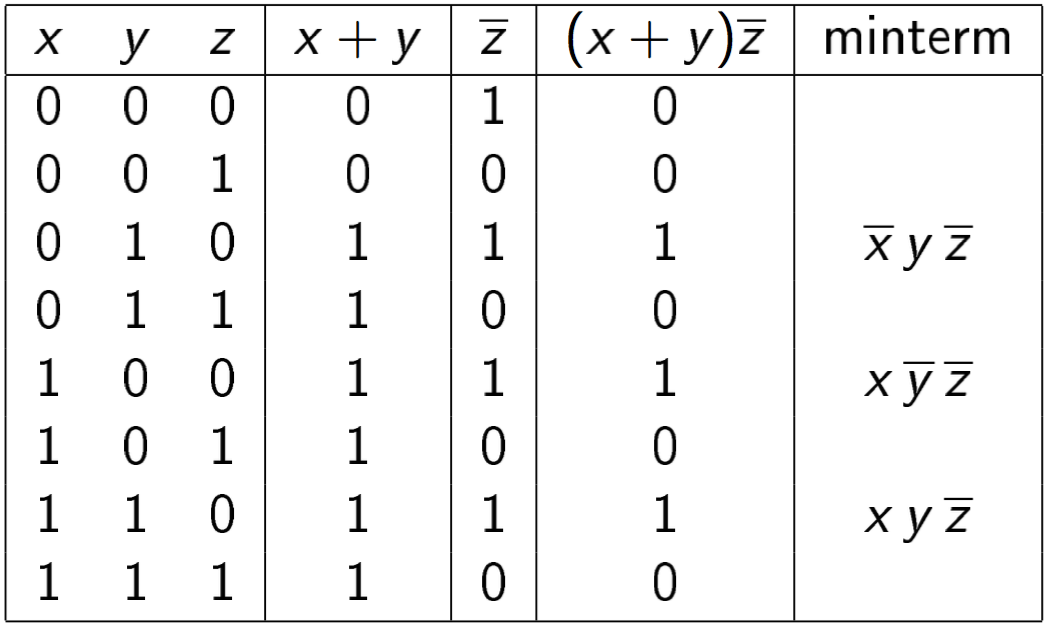
\includegraphics[height=2.4cm]{ex4}
\end{figure}
Los minterms corresponden a las 3 filas de la tabla donde la funci\'on vale 1, as\'i pasa cuando los tres valores valen literalmente 1, por tanto:
\[F(x,y,z) = \bar x y \bar z + x\bar y \bar z + x y \bar z\]
\end{block}
\end{frame}

\begin{frame}
\frametitle{Simplificaci\'on de variables booleanas}
\begin{block}{Ejercicio}
Un motor $M$ est\'a controlado por tres interruptores $x,y,z$ y funciona \'unicamente cuando dos de los interruptores est\'an en modo $ON$. Se deduce la tabla de valores de la funci\'on $M(x,y,z):B^3\longrightarrow B$ y la expresi\'on booleana de $M$ en forma normal disjuntiva. 
\end{block}
\end{frame}


\begin{frame}
\frametitle{Simplificaci\'on de variables booleanas}
\begin{block}{Soluci\'on}
Los tres interruptores son variables booleanes ya que pueden tomar dos valores. Se recuerda que el valor 1 corresponde al interruptor en modo ON y el valor 0 a interruptores en la posici\'on OFF: El motor $M$ toma el valor 1 (encendido) cuando tiene los otros dos interruptores activados y 0 (apagado) en todos los dem\'as casos. 
\end{block}
\end{frame}

\begin{frame}
\frametitle{Simplificaci\'on de variables booleanas}
\begin{block}{Soluci\'on}
La tabla de valores de $M$ a partir de las condiciones del problema son:
 \begin{figure}[h]
  \label{fig:volumen}
\centering
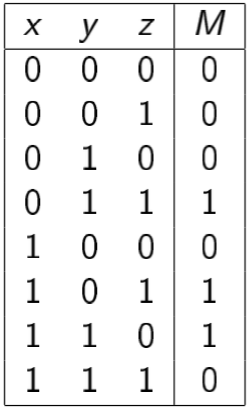
\includegraphics[height=2.6cm]{ex6}
\end{figure}
Y por tanto la expresi\'on booleana $M(x,y,z)$ estar\'a formada por los minterms que hacen que la funci\'on tome el valor 1 (motor encendido):
\[M(x,y,z) = \bar x y z + x\bar y z + x y \bar z\]
\end{block}
\end{frame}




\begin{frame}
\frametitle{Simplificaci\'on de variables booleanas}
\begin{block}{Ejercicios}
Simplificaci\'on de funciones:
\begin{enumerate}
\item $f(x,y) = (x+y)(x+\bar y) (\bar x + y)$
\item $f(x,y,z,w) = \overline{w+w\bar x + yz}$
\item $f(x,y,z,w) = xw+x\bar y + yz + x\bar z$
\end{enumerate}

\end{block}
\end{frame}



\begin{frame}
\frametitle{Simplificaci\'on de variables booleanas}
\begin{block}{Soluciones}

\begin{enumerate}
\item $f(x,y) =xy$
\item $f(x,y,z,w) = \bar x (\bar y + \bar z)$
\item $f(x,y,z,w) =x + yz$
\end{enumerate}

\end{block}
\end{frame}





\begin{frame}
\frametitle{Simplificaci\'on de variables booleanas}
\begin{block}{Diagramas de Karnaugh}
Las funciones booleanas escritas en forma normal disjuntiva se pueden simplificar empleando los diagramas o mapas de Karnaugh. Se trata de un m\'etodo visual muy \'util para realizar simplificaciones. El diagrama de Karnaugh para dos variables $x_1,x_2$ est\'a formado por $2^2 = 4$ cuadrados que representan todos los minterms de grado dos posibles:
 \begin{figure}[h]
  \label{fig:volumen}
\centering
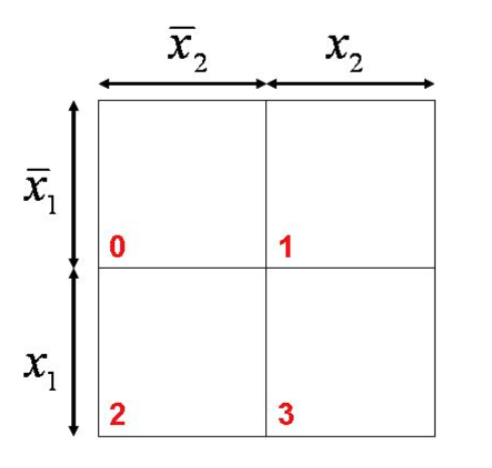
\includegraphics[height=3cm]{k1}
\end{figure}


\end{block}
\end{frame}



\begin{frame}
\frametitle{Simplificaci\'on de variables booleanas}
\begin{block}{Diagramas de Karnaugh}
El diagrama de Karnaugh para 3 variables de $2^3 = 8$ cuadrados:
 \begin{figure}[h]
  \label{fig:volum}
\centering
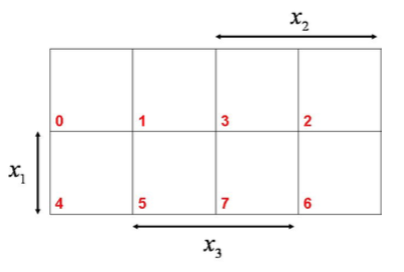
\includegraphics[height=2.8cm]{k2}
\end{figure}
En un diagrama de Karnaugh se dice que dos cuadrados son adyacentes si difieren solo en un literal; es decir, al moverse vertical u horizontalmente solo una variable cambia entre dos cuadrados adyacentes.
\end{block}
\end{frame}


\begin{frame}
\frametitle{Simplificaci\'on de variables booleanas}
\begin{block}{Diagramas de Karnaugh}
En el caso de 4 variables, hay que fijarse en como los valores superiores (los de la izquierda) son adyacentes a los cuadrados inferiores (de la derecha) ya que solo se diferencian en un literal. 
 \begin{figure}[h]
  \label{fig:volumen}
\centering
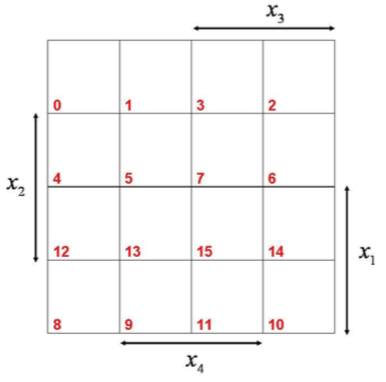
\includegraphics[height=3cm]{k3}
\end{figure}
\end{block}
\end{frame}




\begin{frame}
\frametitle{Simplificaci\'on de variables booleanas}
Las funciones booleanas se pueden representar mediante diagramas de Karnaugh introduciendo a cada cuadrado el valor de la funci\'on. 
\begin{block}{Ejercicios}
Repres\'entese la funci\'on $F$ empleando el diagrama de Karnaugh.
 \begin{figure}[h]
  \label{fig:volumen}
\centering
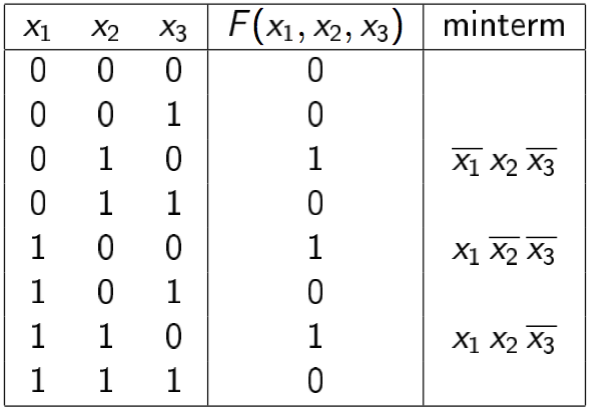
\includegraphics[height=3cm]{k4}
\end{figure}
\end{block}
\end{frame}


\begin{frame}
\frametitle{Simplificaci\'on de variables booleanas}
Las funciones booleanas se pueden representar mediante diagramas de Karnaugh introduciendo a cada cuadrado el valor de la funci\'on. 
\begin{block}{Soluci\'on}
En el diagrama de Karnaugh habr\'a 3 cuadrados con el valor 1, se corresponder\'an con los minterms $\bar x_1 x_2 \bar x_3 = m_2$, $x_1\bar x_2 \bar x_3 ) m_4$ y $x_1x_2\bar x_3 = m6$. La resta de cuadrados tiene el valor 0:
 \begin{figure}[h]
  \label{fig:volumen}
\centering
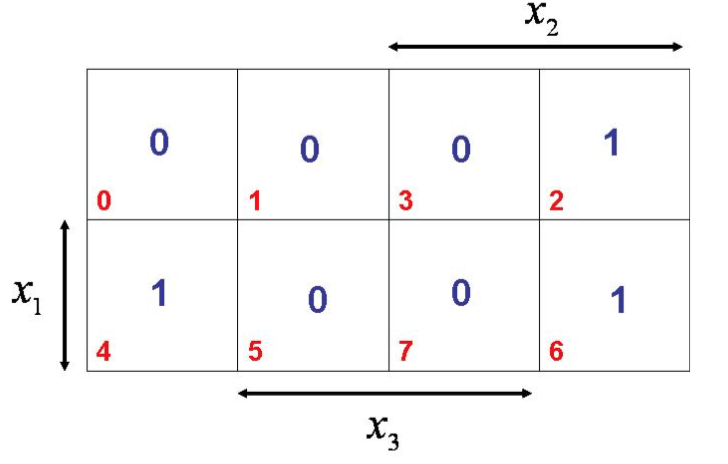
\includegraphics[height=3cm]{k5}
\end{figure}
\end{block}
\end{frame}




\begin{frame}
\frametitle{Simplificaci\'on de variables booleanas}
Para simplificar expresiones booleanas a partir de mapas de Karnaugh se emplear\'a la siguiente regla: siempre que en un diagrama de Karnaugh dos cuadrados adyacentes tomen el valor 1, los minterms representados por los cuadrados de estos se pueden combinar en un producto que contendr\'a solo los literales comunes a los dos minterms.


 \begin{figure}[h]
  \label{fig:volumen}
\centering
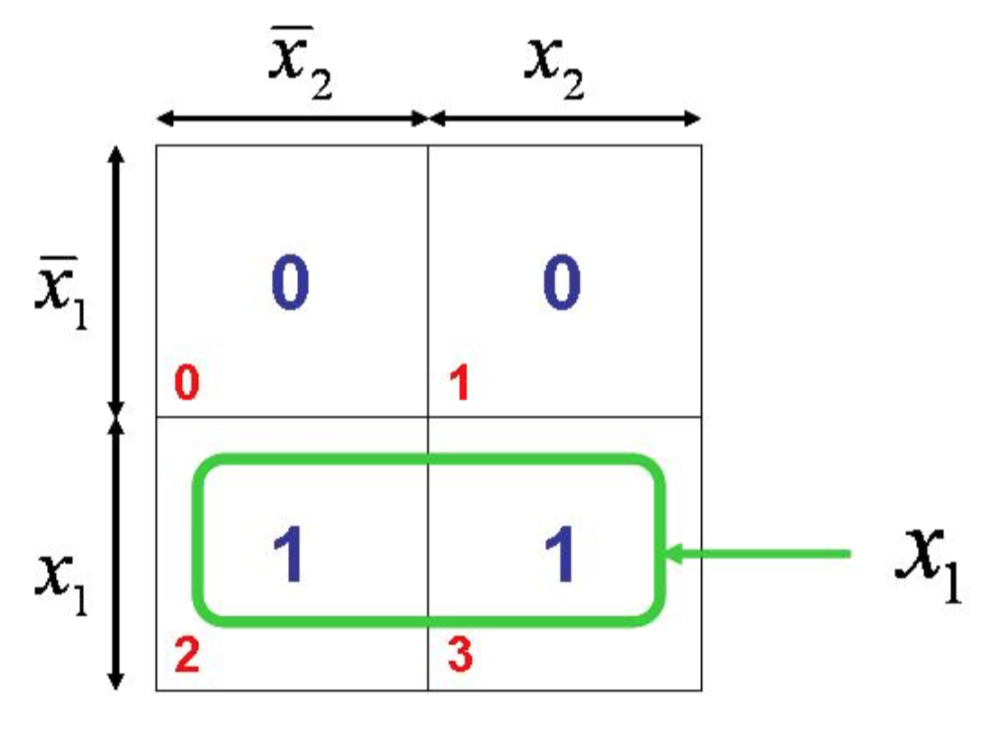
\includegraphics[height=3cm]{k6}
\end{figure}

\end{frame}





\begin{frame}
\frametitle{Simplificaci\'on de variables booleanas}
Esta idea se puede generalizar: se pueden combinar los minterms pertenecientes a cuadrados adyacentes de tal forma que el total de cuadrados combinados sea una potencia de 2. Un bloque formado por un cuadrado elimina 0 variables; un bloque formado por dos cuadrados elimina una variable; un bloque formado por 4 cuadrados elimina dos variables...

 \begin{figure}[h]
  \label{fig:volumen}
\centering
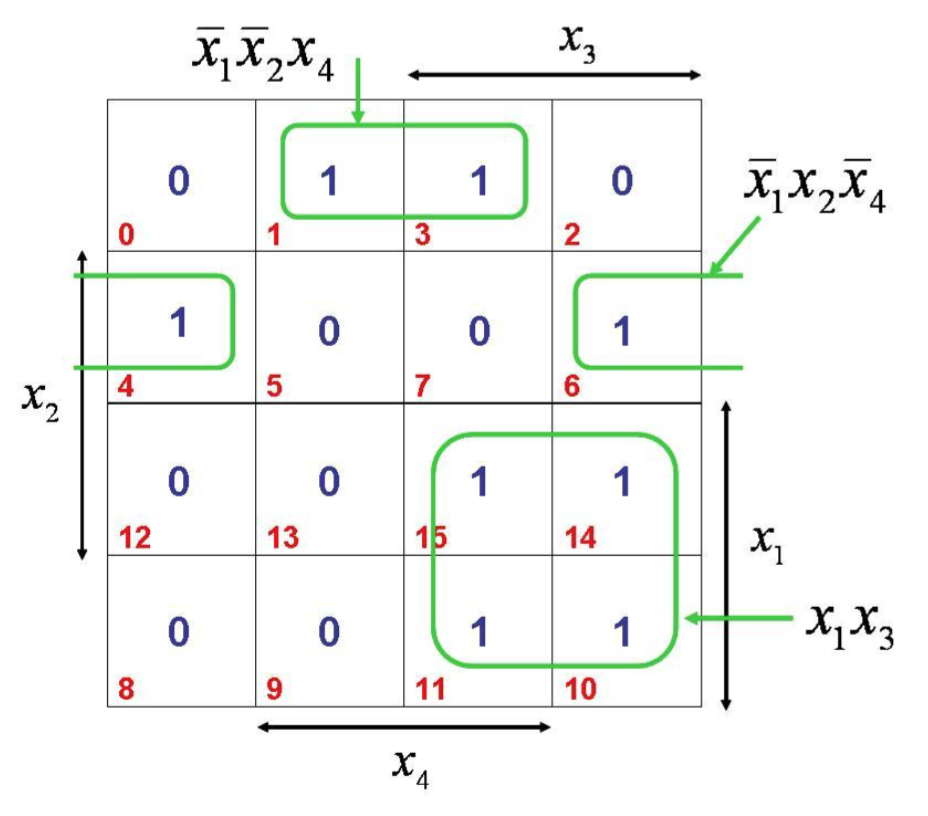
\includegraphics[height=3cm]{k7}
\end{figure}

\end{frame}







\begin{frame}
\frametitle{Simplificaci\'on de variables booleanas}
\begin{block}{Ejercicios}
Simplifica la funci\'on booleana $F(x_1,x_2,x_3)$ del ejemplo anterior emplendo el diagrama de Karnaugh.
\end{block}
 \begin{figure}[h]
  \label{fig:volumen}
\centering
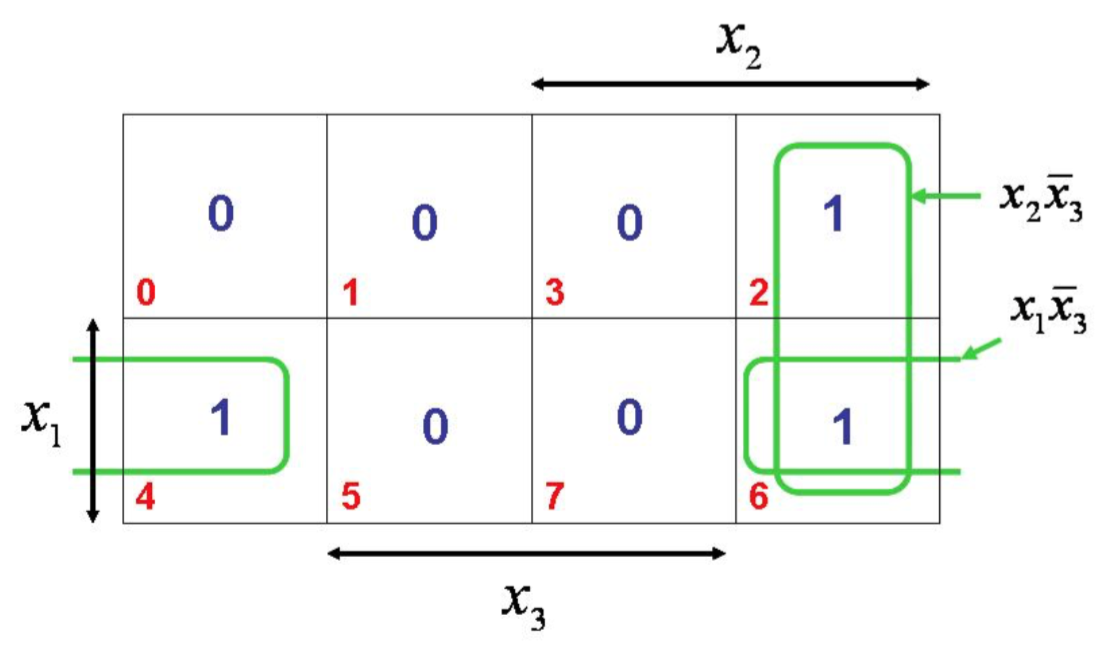
\includegraphics[height=3cm]{k8}
\end{figure}
\[F(x_1,x_2,x_3) = x_2\bar x_3 + x_1\bar x_3\]
\end{frame}



\begin{frame}
\frametitle{Simplificaci\'on de variables booleanas}
\begin{block}{Ejercicio}
Un ascensor dispone de un dispositivo de seguridad: el ascensor funciona cuando est\'e vac\'io o con pesos de entre 25 y 300 kilogramos. El ascensor tiene tres sensores: el sensor A sensible a cualquier peso, el sensor B sensible a pesos superiores a 25 kilogramos y el sensor C sensible a pesos por encima de 300 kilogramos. Encu\'entrese la funci\'on m\'as sencilla que cumple las condiciones expuestas.
\end{block}

\end{frame}






\begin{frame}
\frametitle{Simplificaci\'on de variables booleanas}
\begin{block}{Soluci\'on}
En primer lugar se ha de plantear el problema, identificar variables, la funci\'on booleana y determinar sus valores.

Las variables booleanes $a,b$ y $c$ se corresponen a los tres tipos de sensores y la funci\'on booleana $F$ corresponde al ascensor (se pondr\'a en marcha si se satisfacen las 3 condiciones de seguridad). 

Las variables $a$, $b$ y $c$ toman el valor 1, si detectan peso seg\'un sus l\'imites, y 0 si no detectan peso. 

La funci\'on $F(a,b,c)$ valdr\'a 1 cuando el ascensor se ponga en marcha (se satisfacen las condiciones de seguridad) y 0 cuando no se pone en marcha. 
\end{block}

\end{frame}






\begin{frame}
\frametitle{Simplificaci\'on de variables booleanas}
\begin{itemize}
\item $F(0,0,0) = 1 $, ning\'un sensor detecta peso (el ascensor est\'a vac\'io), el ascensor se pone en marcha. 
\item $F(1,0,0) = 0 $, $A$ detecta peso, pero $B$ y $C$ no detectan peso (teniendo un peso de entre 0 y 25 kg en el ascensor); el ascensor no arranca.  
\item $F(1,1,0) = 1 $, $A$ y $B$ detectan peso pero $C$ no (la carga del ascensor est\'a entre 25 y 300 kg); el ascensor arranca
\item $F(1,1,1) = 0 $, todos los sensores detectan peso ( la carga del ascensor supera los 300 kg); el ascensor no se pone en marcha.
\end{itemize}

\end{frame}




\begin{frame}
\frametitle{Simplificaci\'on de variables booleanas}
 \begin{figure}[h]
  \label{fig:volumen}
\centering
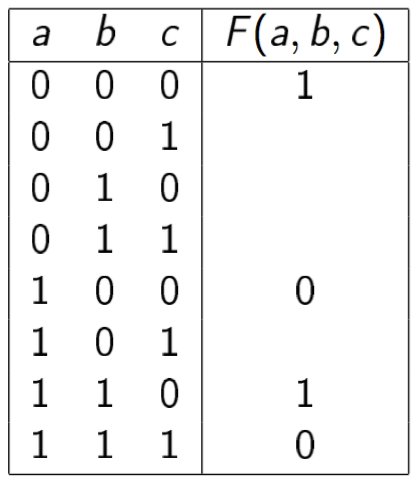
\includegraphics[height=5cm]{k9}
\end{figure}
?`Y para el resta de combinaciones de valores de $a$, $b$ y $c$?
\end{frame}


\begin{frame}
\frametitle{Simplificaci\'on de variables booleanas}
$F(0,1,0)$ corresponde a una situaci\'on donde el sensor $A$ no detecta peso, el sensor $B$ detecta peso entre 25 y 300 kg y el sensor $C$ no detecta peso. Esta es una situaci\'on imposible.
En ciertas ocasiones puede ocurrir que ciertas combinaciones de variables no puedan tomar un valor o que el valor de $F$ no dependa de los valores de sus variables. Estos casos reciben el nombre de \textbf{casos imposibles} o \textbf{indiferentes}. En estas condiciones no importa el valor que tome $F$, y por defecto se le asignar\'a el valor $*$. 
\end{frame}





\begin{frame}
\frametitle{Simplificaci\'on de variables booleanas}
 \begin{figure}[h]
  \label{fig:volumen}
\centering
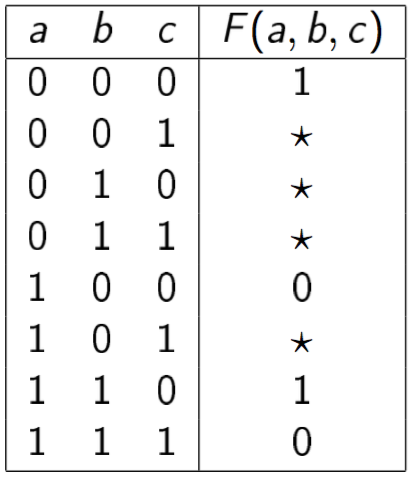
\includegraphics[height=5cm]{k10}
\end{figure}
Una expresi\'on booleana para $F$ es:
\[F(a,b,c) = ab\bar c + \bar a\bar b\bar c\]
\end{frame}



\begin{frame}
\frametitle{Simplificaci\'on de variables booleanas}
El diagrama de Karnaugh es:
 \begin{figure}[h]
  \label{fig:volumen}
\centering
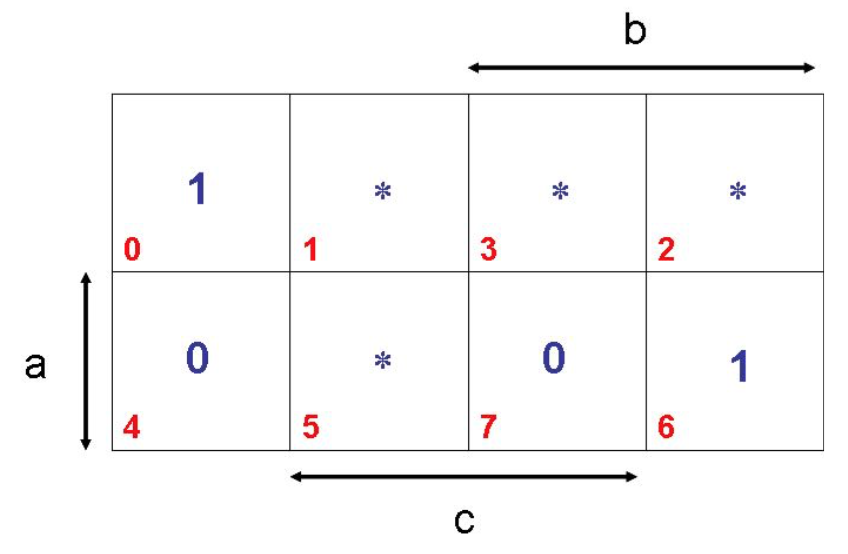
\includegraphics[height=3.2cm]{k11}
\end{figure}
El criterio que se seguir\'a es asignar aquel valor que permita simplificar la expresi\'on definida por el diagrama de Karnaugh. Se obtienen los bloques de mayor tama\~no posible juntando cuadrados que contengan o bien 1 o bien $*$. Los cuadrados correspondientes a situaciones imposibles pueden cubrirse con bloques o quedar al descubierto.
\end{frame}


\begin{frame}
\frametitle{Simplificaci\'on de variables booleanas}
La simplificaci\'on del mapa de Karnaugh es:
 \begin{figure}[h]
  \label{fig:volumen}
\centering
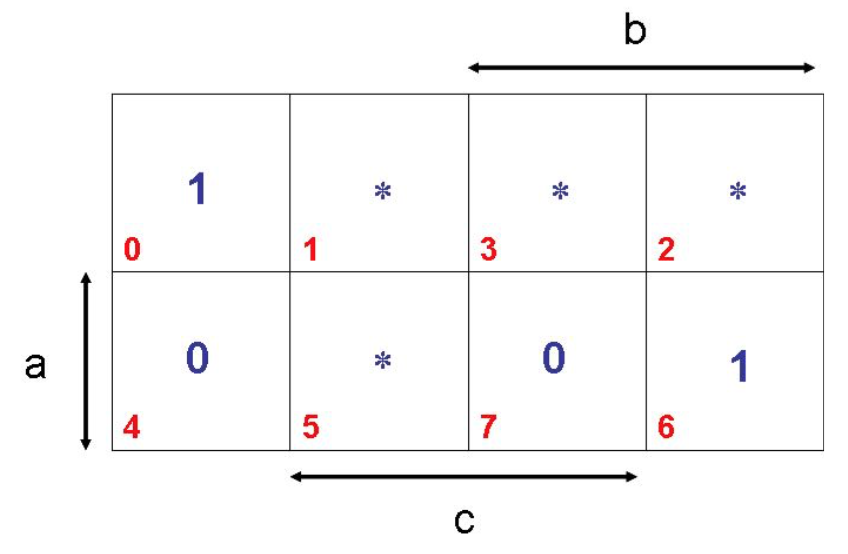
\includegraphics[height=4cm]{k11}
\end{figure}
\[F(a,b,c) = \bar a + b\bar c\]
El ascensor se pone en marcha si el sensor $A$ no detecta peso, o bien si el sensor $B$ detecta peso y el sensor $C$ no. 
\end{frame}
%\begin{tabular}{ |p{1cm}||p{0.8cm}|p{0.8cm}|p{0.8cm}|p{0.8cm}|p{0.8cm}|p{0.8cm}|p{1.6cm}|  }
% \hline
% Z & $x_1$ & $x_2$ & $s_1$& $s_2$ & $v_1$  & $v_2$& Constantes \\
% \hline
%1 &0 & 130 & -100 & 33& 0& -133 & 404 \\
%0 & 0 &  4/3 & -1 & 1/3 & 1 & -1/3 & 4 \\
%0 & 1 & 2/3 & 0 & -1/3 & 0 & 1/3  & 4 \\
% \hline
%\end{tabular}
%\end{frame}


%  \begin{figure}[h]
  %  \label{fig:volumen}
%\centering
%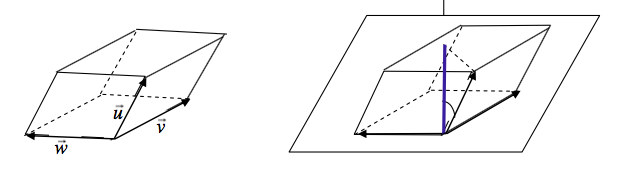
\includegraphics[height=3cm]{volum}
%\end{figure}


\end{document}